%%%%%%%%%%%%%%%%%%%%%%%%%%%%%%%%%%%%%%%%%%%%%%%%%%%%%%%%%%%%%%%%%%%%%%%%%%%%
%% Author template for Management Science (mnsc) for articles with e-companion (EC)
%% Mirko Janc, Ph.D., INFORMS, mirko.janc@informs.org
%% ver. 0.95, December 2010
%%%%%%%%%%%%%%%%%%%%%%%%%%%%%%%%%%%%%%%%%%%%%%%%%%%%%%%%%%%%%%%%%%%%%%%%%%%%
\documentclass[isre,blindrev]{informs3} % current default for manuscript submission
%\documentclass[mnsc,nonblindrev]{informs3}

%%\OneAndAHalfSpacedXI % current default line spacing
%%\OneAndAHalfSpacedXII 
%%\DoubleSpacedXII
\DoubleSpacedXI

% If hyperref is used, dvi-to-ps driver of choice must be declared as
%   an additional option to the \documentstyle. For example
%\documentclass[dvips,mnsc]{informs3}      % if dvips is used
%\documentclass[dvipsone,mnsc]{informs3}   % if dvipsone is used, etc.

% Private macros here (check that there is no clash with the style)

% Natbib setup for author-year style
\usepackage{natbib}
 \bibpunct[, ]{(}{)}{,}{a}{}{,}%
 \def\bibfont{\small}%
 \def\bibsep{\smallskipamount}%
 \def\bibhang{24pt}%
 \def\newblock{\ }%
 \def\BIBand{and}%
 
\usepackage{etoolbox}
\AtBeginEnvironment{quote}{\singlespacing\small}

\usepackage[colorlinks=true,linkcolor=blue,citecolor=blue]{hyperref}%
\usepackage[utf8]{inputenc}
\usepackage[english]{babel}
\usepackage{indentfirst}
\usepackage{amsthm}
\usepackage{caption}
\usepackage{blindtext}
\PassOptionsToPackage{hyphens}{url}\usepackage{hyperref}
\hypersetup{
    colorlinks=true,
    linkcolor=blue,
    filecolor=magenta,      
    urlcolor=cyan,
}
\setlength{\parindent}{24pt}
\setlength{\parskip}{1em}
%% Setup of theorem styles. Outcomment only one.
%% Preferred default is the first option.
\TheoremsNumberedThrough     % Preferred (Theorem 1, Lemma 1, Theorem 2)
%\TheoremsNumberedByChapter  % (Theorem 1.1, Lema 1.1, Theorem 1.2)
\ECRepeatTheorems

%% Setup of the equation numbering system. Outcomment only one.
%% Preferred default is the first option.
\EquationsNumberedThrough    % Default: (1), (2), ...
%\EquationsNumberedBySection % (1.1), (1.2), ...

% For new submissions, leave this number blank.
% For revisions, input the manuscript number assigned by the on-line
% system along with a suffix ".Rx" where x is the revision number.
\MANUSCRIPTNO{ISR-0000-0000.00}

%%%%%%%%%%%%%%%%
\begin{document}
%%%%%%%%%%%%%%%%
%\newtheorem{theorem}{Proposition}
%\newtheorem{corollary}{Corollary}[theorem]
%\newtheorem{lemma}[theorem]{Lemma}
% Outcomment only when entries are known. Otherwise leave as is and
%   default values will be used.
%\setcounter{page}{1}
%\VOLUME{00}%
%\NO{0}%
%\MONTH{Xxxxx}% (month or a similar seasonal id)
%\YEAR{0000}% e.g., 2005
%\FIRSTPAGE{000}%
%\LASTPAGE{000}%
%\SHORTYEAR{00}% shortened year (two-digit)
%\ISSUE{0000} %
%\LONGFIRSTPAGE{0001} %
%\DOI{10.1287/xxxx.0000.0000}%

% Author's names for the running heads
% Sample depending on the number of authors;
% \RUNAUTHOR{Jones}
% \RUNAUTHOR{Jones and Wilson}
% \RUNAUTHOR{Jones, Miller, and Wilson}
% \RUNAUTHOR{Jones et al.} % for four or more authors
% Enter authors following the given pattern:
%\RUNAUTHOR{}

% Title or shortened title suitable for running heads. Sample:
% \RUNTITLE{Bundling Information Goods of Decreasing Value}
% Enter the (shortened) title:
\RUNTITLE{Tethered Durable Goods}

% Full title. Sample:
% \TITLE{Bundling Information Goods of Decreasing Value}
% Enter the full title:
\TITLE{Tethered Durable Goods and Installed Base Degradation via Software Updates: Implications for Product Policy}

% Block of authors and their affiliations starts here:
% NOTE: Authors with same affiliation, if the order of authors allows,
%   should be entered in ONE field, separated by a comma.
%   \EMAIL field can be repeated if more than one author
\ARTICLEAUTHORS{%
\AUTHOR{Snidely Slippery}
\AFF{Department of Bread Spread Engineering, Dairy University, Cowtown, IL 60208, \EMAIL{slippery@dairy.edu}} %, \URL{}}
\AUTHOR{Marg Arinella}
\AFF{Institute for Food Adulteration, University of Food Plains, Food Plains, MN 55599, \EMAIL{m.arinella@adult.ufp.edu}}
% Enter all authors
} % end of the block

\ABSTRACT{%

An installed base of products that are technologically tethered, whether digital products such as smartphones or predominantly non-digital products such as automobiles, can be now degraded in performance through software updates. In this paper we study a monopolist technology vendor{'}s decision to degrade their installed base when they release their newer version. This raises new possibilities and temptations for sellers, and raises new questions not hitherto addressed in the literature on durable goods and innovation, on the optimal product policy for durable goods monopolists. In a two-period setting featuring a monopolist selling a durable good to a unit mass of consumers with uniformly distributed valuation for the good, we first establish that installed base degradation can indeed emerge in equilibrium, with or without innovation, which is consistent with observed industry practice. We establish three novel and surprising results: (i) When consumers in period 1 expect product degradation in period 2, the seller is sometimes better off adopting leasing in period 1, despite having the ability to limit product durability. This reverses the findings from the traditional durable goods literature, where leasing remedies the seller's inability to limit product durability. (ii) The seller engages in "unplanned obsolescence" due to an inability to commit: the seller degrades their version 1 in period 2 (i.e. engages in obsolescence) even though it is profit-improving to avoid degrading. (iii) When consumers in period 1 do not expect and are unaware of the upcoming product degradation in period 2, under some conditions the seller's commitment problem causes them to offer excessive durability. This reverses the findings from the traditional durable goods literature, where the seller's commitment problem causes them to offer insufficient durability. The seller does not face the problem of unplanned obsolescence when consumers are unaware of the upcoming product degradation.

% Enter your abstract
}%

% Sample
%\KEYWORDS{deterministic inventory theory; infinite linear programming duality;
%  existence of optimal policies; semi-Markov decision process; cyclic schedule}

% Fill in data. If unknown, outcomment the field
\KEYWORDS{tethered durable goods, innovation, upgrades, product obsolescence} \HISTORY{This paper was
first submitted in June 2020 and has been with the authors for
__ years for __ revisions.}

\maketitle
%%%%%%%%%%%%%%%%%%%%%%%%%%%%%%%%%%%%%%%%%%%%%%%%%%%%%%%%%%%%%%%%%%%%%%

% Samples of sectioning (and labeling) in MNSC
% NOTE: (1) \section and \subsection do NOT end with a period
%       (2) \subsubsection and lower need end punctuation
%       (3) capitalization is as shown (title style).
%
%\section{Introduction.}\label{intro} %%1.
%\subsection{Duality and the Classical EOQ Problem.}\label{class-EOQ} %% 1.1.
%\subsection{Outline.}\label{outline1} %% 1.2.
%\subsubsection{Cyclic Schedules for the General Deterministic SMDP.}
%  \label{cyclic-schedules} %% 1.2.1
%\section{Problem Description.}\label{problemdescription} %% 2.

% Text of your paper here

\section{Introduction}

In 2018, Apple was accused of deliberately slowing down older versions of iPhones. The mechanism for this was through updates to the iOS operating system, pushed to consumers' phones via the internet. After much controversy, Apple confirmed this. However, the business press was critical of Apple's lack of transparency, and raised questions about Apple's ability to guarantee battery quality for a reasonable period of time, as seen from a recent Forbes article:\footnote{https://www.forbes.com/sites/ewanspence/2017/12/20/apple-iphone-kill-switch-ios-degrade-cripple-performance-battery/} 
\begin{quote}{``}Following significant examination and documentation
by third parties, Apple has confirmed that its software does degrade the performance of older iPhones. This is, according to the statement, undertaken
in {`}a bid to deliver the best experience for its customers{'}. That may be the case, but it is a trick that Apple has not been open about...Apple has implemented this for iPhone 7 users, a phone that was announced just over fourteen months ago and arguably was still Apple’s leading smartphone just four months ago. Can Apple really not guarantee battery performance for that length of time?{''}
\end{quote}

This highlights an important new possibility with regard to durable goods: many durable goods are tethered to the vendor in the sense that the vendor can push software updates that affect the performance of the existing installed base of products. This is not limited to smartphones, but also cars such as the Tesla. 

Part of the reason why an older phone slows down is because its battery is getting older, as Apple points out. Part of the reason may be that the updated operating system, which needs to be updated to handle newer capabilities (such as security patches for newly identified vulnerabilities), can end up slowing the older hardware in the older phones. However, part of the reason could also be that the seller wants users to upgrade to the newer version. It is difficult to ignore the financial incentive for firms to do so.

In this paper, we focus on this third aspect, and examine whether a seller faces incentives to degrade the installed base of products in order to induce consumers to switch to newer versions. We consider a two-period model, where the seller sells to a mass of consumers in period 1. This is referred to as the installed base in period 2. The seller in period 2 can choose to degrade their installed base of products, to induce the previous-period buyers to buy again in period 2. We show that a durable goods monopolist can realize a higher profit when they degrade or disable the performance of their installed base in period 2, whether or not the newer version is innovative compared to the older version. Surprisingly, we show that under some conditions, the seller may be tempted to degrade their installed base in period 2 even if it is sub-optimal
for their profit. Companies such as Apple may be facing a temptation to degrade their older version in subsequent periods, even though that does not optimize their profit. We then find that under some conditions, the seller has to adopt leasing despite being able to degrade their installed base, which is in contrast to prior literature where the seller adopts leasing because they can't degrade their installed base \citep{stokey_rational_1981, bulow_durable-goods_1982, bhaskaran_selling_2005}.
We also find that if the buyer in period 1 does not expect the seller to degrade their installed base in period 2, then the seller's commitment problem prevents them from optimal sales of the new version, and it leads them to offer excessive durability of the previous version, which is in contrast to prior results in the durable goods literature where the seller's commitment problem leads to diminished durability of the previous version, either through producing less-durable products in the first period \citep{bulow_durable-goods_1982}, style changes \citep{waldman_new_1993} or through network effects \citep{ellison_neo-luddites_2000, sankaranarayanan2007innovation}. 

In the industry examples discussed above, degradation is not complete - a customer can still (barely) use their older iPhone, even though it is significantly
slower. However, for practical purposes, the slow response of the iPhone wears on the customer, and they eventually yield and buy the new iPhone.
Our analysis captures this notion, and models the degradation of the installed base as a complete degradation - i.e. in period 2, when the seller
degrades the installed base, its utility decreases to zero.

\section{Literature}

To better understand the questions raised by the Apple incident, we draw upon the literature on durable goods \citep{coase_durability_1972, stokey_rational_1981}, product obsolescence \citep{bulow_economic_1986, waldman_new_1993}, technological innovation \citep{dhebar_durable-goods_1994, kornish_pricing_2001}, damaged durable goods \citep{deneckere_damaged_1996, hahn_damaged_2006}, and leasing \citep{bhaskaran_selling_2005}, and extend it to the context of tethered durable goods. As mentioned in the previous section, we explore whether durable goods vendors have an incentive to degrade their installed base in a subsequent period when they do or don't release newer versions. We find that under some conditions, incentives to degrade the installed base exist. We also show that there exist some conditions when the profit is actually higher without degrading than with, but the seller faces a commitment problem
and ends up degrading their installed base despite the damage to their profitability. Another novel finding is that the seller is hampered by (somewhat different) commitment problems when they degrade their installed base, as well as when they don't.

When a durable goods vendor introduces an upgrade, prior literature has shown that if the technology is changing too rapidly and the vendor is unable to commit to future prices for the upgrade, no equilibrium strategy exists \citep{dhebar_durable-goods_1994}. This problem is mitigated if the vendor can offer a uniform price for the upgrade to buyers who are upgrading from the older version, as well as first-time buyers of the upgrade \citep{kornish_pricing_2001}. With tethered durable goods, we show that even if the vendor commits to offering a uniform price for the upgrade as done by \cite{kornish_pricing_2001}, there exists a region with intermediate level of innovation where the optimum product policy is not an equilibrium strategy as in \cite{dhebar_durable-goods_1994} because the seller faces a commitment problem with regard to optimizing their upgrade pricing.

Durable goods vendors face a commitment problem \citep{coase_durability_1972, bulow_durable-goods_1982}, because durable
goods sold in future periods affect the value of goods sold in prior periods. This limits the seller{'}s profits \citep{stokey_rational_1981}. Prior literature has examined leasing as a remedy for the seller's commitment problem \citep{bulow_durable-goods_1982, bhaskaran_selling_2005}. However, most of the literature on leasing durable goods does not address the question of leasing in the context of upgrades. Our paper finds that with durable goods upgrades, under some conditions the seller is strictly better off leasing to avoid a sub-optimal profit outcome, whereas in other conditions, the seller's equilibrium selling strategy is equivalent to leasing. Further, with tethered durable goods, we find that the seller's ability to degrade their installed base does not mitigate the commitment problem identified by \cite{coase_durability_1972} and  \cite{bulow_durable-goods_1982}, but makes it more pronounced.

Prior work has modeled changes to product durability as either (a) ex ante planned obsolescence, wherein firms produce {``}durable{''} goods with uneconomically short lives, which break down earlier than they should
\citep{bulow_economic_1986}  - so as to induce customers to make repeat purchases, or (b) ex post planned obsolescence \citep{waldman_new_1993}, wherein a vendor can introduce newer versions whose very presence can obsolete the older versions due to fashion (e.g. newer model cars putting older models out of fashion) or technological incompatibility (newer version of a software causing older versions to become unable to open files produced by the newer version), and so on. 

Tethered durable goods offer vendors an opportunity (or temptation) that is not adequately captured by either of the above two theoretical lenses. The vendor can reduce the economic life of their installed base of products as in (a) above, but do so ex post (in a later period) as in (b) above. When the vendor is able to set the economic life of their product prior to its release, as in (a), that gives the vendor a measure of control and helps them avoid time inconsistency problems. When the vendor is able to do an ex post planned obsolescence as in (b), they are required to produce an improved version, in order to obsolete their previous version. However, with tethered durable goods, when the vendor can obsolete their older version after it has been released and is in use by their customers, this subjects the vendor to a time inconsistency problem (unlike (a)), while letting them avoid the discipline of innovating (unlike (b)). In this paper, we take a comprehensive look at the vendor's optimal product policy in the light of this changed situation.

In \cite{waldman_new_1993}  planned obsolescence is the result of innovation. The greater the incremental value, greater the planned obsolescence of the previous version. In our case, from an economic and marketing viewpoint, there is a major difference: if the seller can degrade performance with software based updates, then product obsolescence is delinked from the incremental value delivered by the newer product. The seller can degrade the previous version (installed base) even without providing any incremental value in the subsequent period. This novel feature of tethered durable goods can be better understood by mapping the optimality of product obsolescence by varying the incremental value. 

Incremental value can be decomposed into two dimensions: one is the incremental value of the new version compared to the older version, and the other
is the incremental value of the older version relative to the marginal cost. We leverage both these dimensions for enhanced insight, and explore
the optimality of the decision to degrade, in a parameter space with varying levels of incremental innovation (high versus low) and varying levels
of { }intrinsic product value relative to marginal cost (again, high versus low). Surprisingly, we find that under some conditions, this obsoleting
of the prior version actually hurts the seller{'}s profit - they are better off not engaging in this action, but may lack the ability to commit to
the optimal decision.

The phenomenon of selling damaged durable goods has been studied before \citep{deneckere_damaged_1996,hahn_damaged_2006}. \cite{hahn_damaged_2006} studies damaged goods
- i.e. the main product offered as a crimped version, offered simultaneously with the main version, or sequentially after the main version - can
help alleviate the Coasian time inconsistency problem. Another way to eliminate the competition between different versions of durable goods, is to
damage or disable the previous version when the new version is introduced. Our work explores this aspect by studying durable goods that are rendered
completely unusable (rather than partially damaged) in future periods, when new versions are introduced. 

\section{Outline of analysis}\label{outline}
We consider the standard two-period model commonly employed in the durable goods literature \citep{xin2018impact, jia_selling_2018, mehra_competitive_2012, bhaskaran_selling_2005, kornish_pricing_2001, ellison_neo-luddites_2000, dhebar_durable-goods_1994}, featuring a monopolist durable goods vendor selling to a unit mass of vertically differentiated consumers with heterogeneous and uniformly distributed valuations for the product. In period 1, the seller chooses an optimal price for their product, which results in a cutoff consumer such that all consumers with valuations higher than this cutoff purchase the product. In period 2, the seller could offer the same product without innovation (section \ref{no-innovate}), or the seller could innovate and introduce an upgrade (section \ref{innovate}). 

Table \ref{varlist} lists the variables in the model.

\begin{center}
\captionof{table}{List of variables}\label{varlist}
\\
\\
\begin{tabular}{ |l|l| }

\hline
 \(v_1\) & \text{Product value in period 1} \\
 \(v_2\) & \text{Product value in period 2 \((v _2 > v _1)\)} \\
 \(v\) & \text{Product value in either period in no-innovation case} \\
 \theta _i & \text{Customer type, uniformly distributed in [0,1]}\\
 \(p_i\) & \text{Product price in period, where i \(\in\) \{1,2\}}  \\
 \pi _i & \text{Seller profit in period, where i \(\in\) \{1,2\}} \\
 \pi _{12} & \text{Seller profit in period 2 from selling to those who upgrade from period 1} \\
 \(c\) & \text{Marginal product cost per unit sold, assumed same for both versions}
\\
\hline

\end{tabular}
\end{center}
\\
\\
\vspace{2em}
\par
In either case, the second period sales faces competition from the first period installed base, and conversely, anticipation of lower future prices causes consumers to hold off on first period purchases \citep{coase_durability_1972, ellison_neo-luddites_2000, kornish_pricing_2001}. We incorporate this feature in our model: in period-2, consumers compare their value from buying to their value from continuing to use the older version, where available. The first-period buyers weigh their benefit from buying in period 1, versus waiting and buying from period 2. 

We first analyze the case where the monopolist does not innovate (section \ref{no-innovate}). We first compute their profits from a no-degrade policy (section \ref{no-innovate-no-degrade}), and then their profits from a degrade-policy (section \ref{no-innovate-degrade}). We find that mostly, as at the start of the two-period time horizon,
the seller is better off not degrading product quality (section \ref{no-innovate-compare-overall}), but in period 2, the seller is tempted to degrade the product quality (section \ref{no-innovate-compare-period-2}). We then super-impose the no-degrade and degrade policies, and derive overall results for the no-innovation case (section \ref{no-innovate-superimpose}).

Next, we analyze the case where the monopolist does innovate (section \ref{innovate}). Here, we first compute the seller{'}s profit when they don{'}t degrade their initial version in period 2 (section \ref{innovate-no-degrade}). Then we compute their profit when they degrade (section \ref{innovate-degrade}). In this section, we find a novel kind of commitment problem for the seller (proposition \ref{prop1}). We then compare the seller's overall profit (section \ref{innovate-compare-overall}) and period-2 profit (section \ref{innovate-compare-period-2}) with and without degradation. We super-impose the no-degrade and degrade policies, and derive overall results for the innovation case (section \ref{innovate-superimpose}). Contrary to the no-innovation case, in the innovation-case when the seller is incentivized to degrade their installed base in period 2, their profit is mostly optimized, which can partially explain the incentives behind recent behavior by Apple. However, there does exist a smaller region with suboptimal overall profit, highlighting a commitment problem that durable goods vendors should be aware of. We find that the seller is now forced to lease, even though they can degrade their installed base. Next, we perform a similar analysis, but this time assuming that consumers in period 1 are not aware of the seller's intention to degrade the installed base in period 2 (section \ref{innovate-no-degrade-unaware}). We now find that (a) the seller is better off keeping consumers unaware of the upcoming product degradation, than let them become aware of it (proposition \ref{prop2}), and (b) under some conditions, the seller is constrained to offer excessive durability of the previous version.


\section{When monopolist does not innovate}\label{no-innovate}

Here we consider the base case when the product involves no innovation, but is sold over two periods. We show that when the durable good is not subject
to innovation, and when \(v>>c\) (specifically, \(v>10c\)) it is better for monopolist to degrade the product after each period, rather than not
(i.e. \(\left.\pi _n<\pi _d\right)\). However, at the start of each period, the seller is subject to a different set of incentives: { }(i) at the
start of period 1, when \(10c>v>c\), the monopolist is better off not degrading the product in period 2 (i.e. \(\pi _n>\pi _d\)); nevertheless (ii)
in period 2, when \(v>\frac{5}{4}c\), the monopolist faces incentives in period 2, to crimp their product so as to encourage more sales (i.e. \(\pi
_{\text{d2}}>\pi _{\text{n2}}\)). Combining the two analyses, we find that in figure \ref{fig:fig3}, in region (I), when \(v>10c\), we have \(\pi _n<\pi _d\)
and \(\pi _{\text{n2}}<\pi _{\text{d2}}\), so that it is always optimal for the seller to degrade. In region (II), when \(10c>v>\frac{5}{4}c\), we
have \(\pi _n>\pi _d\) and \(\pi _{\text{n2}}<\pi _{\text{d2}}\), so that it is optimal for the seller to not degrade their first-period product
in period 2, but at the start of period 2 the seller nevertheless faces an incentive to degrade their initial version, forcing consumers to purchase
the same product again. Rational forward looking consumers expect this behavior, and it decreases their willingness to pay in period 1. In region
(III), when \(\frac{5}{4}c>v>c\), { }we have \(\pi _n>\pi _d\) and \(\pi _{\text{n2}}>\pi _{\text{d2}}\), so that it is optimal for the seller to
not degrade their product, either in period 1 or period 2. In the no-innovation situation, it is never the case that (\(\pi _n<\pi _d\) and \(\pi
_{\text{n2}}>\pi _{\text{d2}}\)) - i.e. that the seller is overall better off degrading their product, but faces an incentive to not degrade in period
2. (As we will see later, this last condition does not hold for the case of innovation.)

Our analysis in this section proceeds as follows. Section 5.1 (case A) derives the seller{'}s overall profit and period-2 profit when they sell \(v\)
in period 1, and does not degrade it in period 2 (i.e. the period 1 product can be used for two periods). Section 5.2 (case B) computes the seller{'}s
overall profit and period-2 profit when they sell v in period 1, but degrade it in period 2, so that it can only be used for one period. We compare
the overall profits and period-2 profits under the above conditions, to derive regions (see figure \ref{fig:fig3}) where (I) \(\pi _n<\pi _d\) and \(\pi
_{\text{n2}}<\pi _{\text{d2}}\), (II) \(\pi _n>\pi _d\) and \(\pi _{\text{n2}}<\pi _{\text{d2}}\), and (III) \(\pi _n>\pi _d\) and \(\pi _{\text{n2}}>\pi
_{\text{d2}}\), and discuss findings and implications.

\subsection{Case (A): Monopolist does not degrade period-1 bought v in period 2}\label{no-innovate-no-degrade}

Since the product purchased in period 1 continues to be useful in period 2, period-1 buyers will continue to use it in period 2. Since there is no
innovation, consumers \(\left[\theta _1,1\right]\) who bought in period 1 will not buy in period 2. Some \(\left.\left[\theta _2,\theta _1\right.\right)\)
customers who bought nothing in period 1 will buy v in period 2.

In period 2, the threshold customer \(\theta _2\) is indifferent between (buying v at price \(p_2\)) and (buying nothing), which is given by the
indifference equation \(\theta _2v-p_2=0\). We set the seller{'}s optimal \(p_2=v \theta _2\) in the seller{'}s second period profit \(\pi _2=\left(p_2-c\right)\left(\theta
_1-\theta _2\right)\), and solve the first order condition \(\frac{\partial \pi _2}{\partial \theta _2}=0\) to obtain the optimal \(\theta _2^*=\frac{c+v
\theta _1}{2 v}\).

In period 1, the threshold customer \(\theta _1\) is indifferent between (i) buying v at price \(p_1\) and using it for two periods, and (ii) waiting,
and buying v at price \(p_2\) in period 2. This implies the following indifference equation: \(\theta _1 (2 v) - p_1 = \theta _1 v - p_2\), which
yields the optimal \(p_1=\frac{1}{2} \left(c+3 v \theta _1\right)\). We substitute for this \(p_1\) in the seller{'}s optimal period-1 profit \(\pi
_1=\left(p_1-c\right)\left(1-\theta _1\right)\). 

The overall profit (subscript {``}n{''} to denote that case that the seller is not degrading the older version) is given by the sum of the profit
over each period: \(\pi _n=\pi _1+\pi _2\). Solving the first order condition \(\frac{\partial \pi _n}{\partial \theta _1}=0\) for the optimal \(\theta
_1\) that maximizes overall profit over both periods, we obtain \(\theta _1=\frac{3}{5}\), and \(\theta _2=\frac{3}{10}+\frac{c}{2 v}\). We now substitute
the optimal \(\theta _1\) and \(\theta _2\) values into the profit expression to compute the total optimal profit, over both periods:
\begin{equation}\label{pi_n_no_innov_no_degrade}
\pi _n=\frac{1}{20} \left(-10 c+\frac{5 c^2}{v}+9 v\right)
\end{equation}
We then use the optimal $\theta $ values to compute the second-period profit expression:
\begin{equation}\label{pi_n2_no_innov_no_degrade}
\pi _{\text{n2}}=\frac{(5 c-3 v)^2}{100 v}
\end{equation}
Both of the above profit expressions are subscripted by {``}n{''} to refer to the case where the seller does not degrade the older version in the
second period.

\subsection{Case (B): Monopolist does degrade v}
\label{no-innovate-degrade}

This time, we consider the case when the monopolist does degrade v in period 2. As before, we proceed with period 2 analysis first. Since the seller depreciates \(v\) in period 2, customers who bought \(v\) in period 1 will buy
\(v\) again in period 2. In each period, there is only one cutoff customer: \(\theta _1\) in period 1, and \(\theta _2\) in period 2. We show that,
since \(v_2=v_1\), it follows that \(\theta _2=\theta _1\) as well. The threshold customer \(\theta _2\) is indifferent between (i) buying v at price
\(p_2\) and (ii) buying nothing, which yields the following indifference equation: \(\theta _2v-p_2=0\). Solving for \(p_2\) yields { }\(p_2=v \theta
_2\), which we substitute in the seller{'}s second period profit: \(\pi _2=\left(p_2-c\right)\left(1-\theta _2\right)\). Solving the first order
condition \(\frac{\partial \pi _2}{\partial \theta _2}=0\) yields the optimal \(\theta _2=\frac{c+v}{2 v}\), which yields the second period profit
\(\pi _{\text{d2}}\) (we now append the subscript {``}d{''} to denote that this is the case where the seller degrades the initial version in period
2):
\begin{equation}\label{pi_d2_no_innov_degrade}
\pi _{\text{d2}}=\frac{(v-c)^2}{4 v}
\end{equation}
The first period is no different from the second period, in that the product v sold in period 1 at price \(p_1\) will be used only for one period.
The buyer will (by construction) degrade it in period 2, and consumers will expect it to be degraded. Hence, \(p_1=p_2\), and hence \(\theta _1=\theta
_2\). Therefore, the seller chooses \(p_1=\frac{c+v}{2}\), and optimizes their first period profit \(\pi _1=\left(p_1-c\right)\left(1-\theta _1\right)\).
Solving the first order condition \(\frac{\partial \pi _1}{\partial \theta _1}=0\) for optimal \(\theta _1\), we get \(\theta _1=\frac{c+v}{2 v}\).
Substituting \(p_1\), \(\theta _1\) into the expression for \(\pi _{\text{d1}}\), we get 
\begin{equation}
\pi _{\text{d1}}=\frac{(v-c)^2}{4 v}
\end{equation}
The overall profit therefore is 
\begin{equation}\label{pi_d_no_innov_degrade}
\pi _d =\pi _{\text{d1}}+\pi _{\text{d2}}=\frac{(v-c)^2}{2 v}
\end{equation}
\subsection{Comparison of overall profit for the two cases}
\label{no-innovate-compare-overall}

Comparing equations \ref{pi_n_no_innov_no_degrade} and \ref{pi_d_no_innov_degrade} for \(\pi _n\) and \(\pi _d\) respectively (shown below), from the point of view of maximizing overall profit:
\(\pi _n>\pi _d\) when \(10 c>v>c\) (region (II) in figure \ref{fig:fig1}), suggesting that with no innovation, at the start of period 1, there exists
a range of intermediate parameter values where it is optimal for the seller to refrain from degrading their first-period product in period 2. In
other words, when the marginal cost c is somewhat large compared to product utility v (to the highest type customer), the seller is { }better off
not degrading when the product is subject to no innovation. (For example, an iPhone costs about $\$$370, and retails for about $\$$1000).

\begin{figure}[htp]
    \centering
    \includegraphics[width=9cm]{2020_05_19-overleaf-mirror_gr1.pdf}
    \caption{Comparison of overall profit. Region I: \(\pi _{\text{n}} < \pi _{\text{d}}\), Region II: \pi _{\text{n}} > \pi _{\text{d}} }
    \label{fig:fig1}
\end{figure}

However there exists a small region (I) (figure \ref{fig:fig1}) with very low marginal cost relative to product value (\(v>10 c\)) , where it is better
for overall profit for the seller to degrade the period-1 version in period 2. This corresponds to the classic leasing result in durable goods literature.
In the case of software, this suggests the use of subscription.

Region (III) (figure \ref{fig:fig1}) is infeasible because the value of the product to the customer with the highest valuation \((\theta =1)\) is lower
than the marginal cost: \(v<c\).

We depict the results for the parameter regions as follows:
\begin{equation}
\pi _n>\pi _d \forall \{9 c> v>c\}
\end{equation}
\begin{equation}
\pi _n<\pi _d \forall \{v>10c\}
\end{equation}
There is a region {\{\(10 c > v> 9 c\)\}} where the result is indeterminate.

\subsection{Period 2 profit comparison for the two cases}
\label{no-innovate-compare-period-2}

Comparing equations \ref{pi_n2_no_innov_no_degrade} and \ref{pi_d2_no_innov_degrade}, it can be shown in region (I) of figure \ref{fig:fig2}, that when \(v>\frac{5}{4}c\), we have \(\pi _{\text{n2}}<\pi _{\text{d2}}\),
suggesting that with no innovation, at the start of period 2, the seller faces a temptation to degrade the version 1 in period 2: their profit from
degrading in period 2 \(\left(\pi _{\text{d2}}\right.\)) exceeds their profit from not degrading in period 2 \(\left(\pi _{\text{n2}}\right.\)).

\begin{figure}[htp]
    \centering
    \includegraphics[width=9cm]{2020_05_19-overleaf-mirror_gr2.pdf}
    \caption{Comparison of period-2 profit. Region I is where \pi _{\text{n2}} < \pi _{\text{d2}} }
    \label{fig:fig2}
\end{figure}

In region (II) of figure \ref{fig:fig2}, when \(c<v<\frac{5}{4}c\), we have \(\pi _{\text{n2}}>\pi _{\text{d2}}\) : at lower levels of value relative to
marginal cost, it does not make sense for the seller to degrade the installed base in period 2. 

We depict the results for the parameter regions as follows:
\begin{equation}
\pi _{\text{n2}}<\pi _{\text{d2}} \forall \left\{v > \frac{5}{4}c \right\}
\end{equation}
\begin{equation}
\pi _{\text{n2}}>\pi _{\text{d2}} \forall \left\{\frac{5}{4}c>v > c \right\}
\end{equation}
\subsection{Superimposing optimal actions of both periods}
\label{no-innovate-superimpose}
Superimposing figure \ref{fig:fig1} and figure \ref{fig:fig2} in figure \ref{fig:fig3}, we find that when the product utility v (to the highest type customer) vis-a-vis the marginal cost is in the range
\(\frac{5}{4}c<v<10c\) (region II), the seller faces a commitment problem: at the start of period 2, the seller is { }better off degrading the installed base
in period 2, whereas at the start of period 1, the seller is better off preserving the installed base in period 2. In the range \(v>10c\) (region I), the seller
faces uniform incentives - in period 1 and period 2 - to degrade the installed base in period 2. In both of the above cases, the observed outcome
is that the seller degrades the installed base in period 2, which is consistent with observed practice in industry.

\begin{figure}[htp]
    \centering
    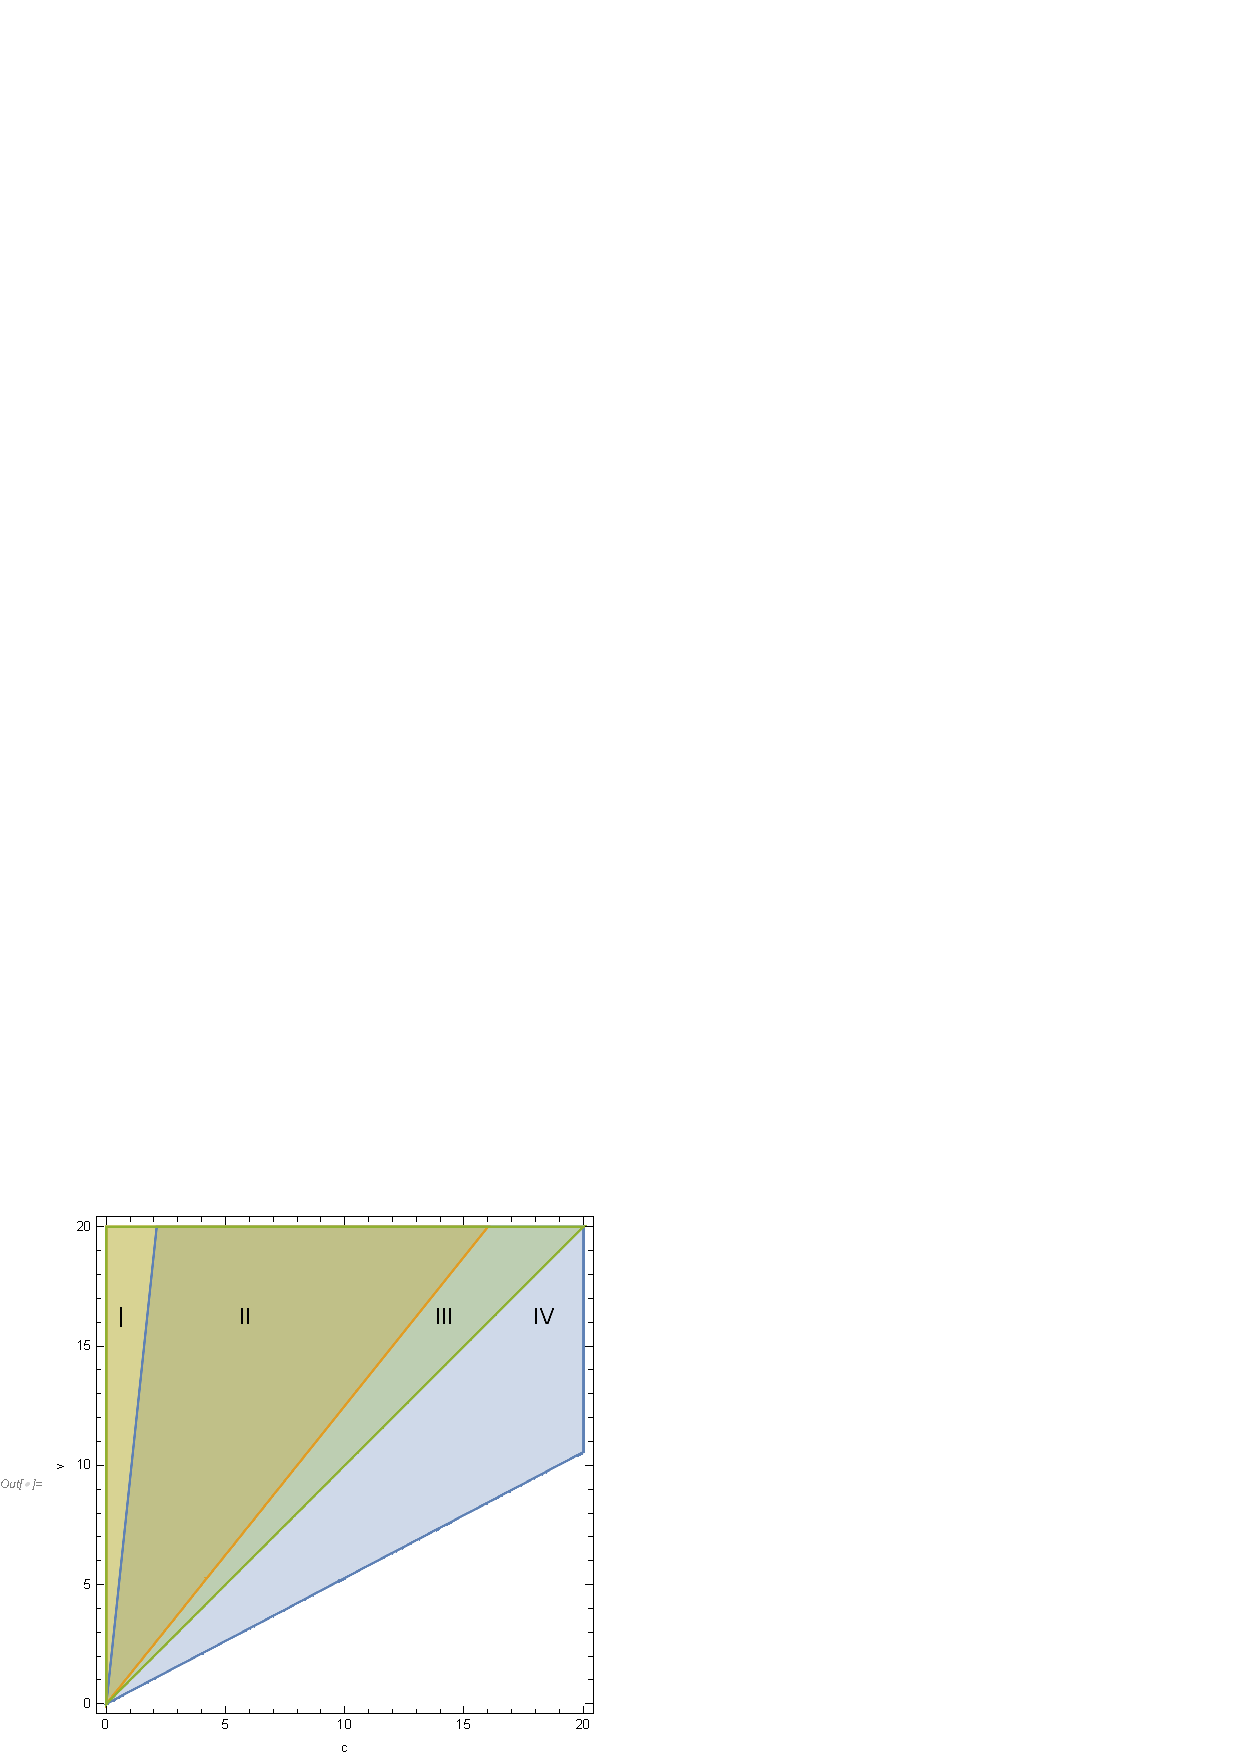
\includegraphics[width=9cm]{2020_05_19-overleaf-mirror_gr3.pdf}
    \caption{Comparison of overall profit as well as period-2 profit}
    \label{fig:fig3}
\end{figure}

However, when \(c<v<\frac{5}{4}c\) (region III), the seller again faces uniform incentives - in period 1 and period 2 - to preserve the installed base in period
2, while continuing to sell to newer customers in period 2. For this smaller region, when v is not much larger than c, in the second period it is
not optimal to depreciate the older version. (Region IV is not of interest because here, marginal cost c is higher than product value v.)

This analysis therefore throws light on why sellers might sometimes act to degrade their installed base, and at other times act to preserve their
installed base.

\pmb{Results - case of no-innovation:}

Region I: At high intrinsic value relative to marginal cost, the seller is better off degrading the product in period 2, as at the start of period 1 as well as period 2. Degrading the product is optimal in both first and second periods. Here, leasing is not required, but is equivalent to the observed outcome from sale.

Region II: At moderate intrinsic value relative to marginal cost, we observe that the seller is better off not degrading their product in period 2, as at the start of period 1, but at the start of period 2 they face a temptation to degrade their product. Consumers expect this outcome and lower their willingness to pay for the initial version, and this hurts the seller{'}s
profit. This is a variant of the commitment problem identified in the durable goods literature \citep{waldman_new_1993, ellison_neo-luddites_2000}. This prior work has identified the existence of the commitment problem in the presence of innovation, while here we show that this commitment problem exists even in the absence of innovation. Leasing \citep{bulow_durable-goods_1982} will not cure this because leasing will restrict the first period good's usage to one period, whereas the optimal usage is two periods.

Region III: Seller is better off not degrading their product in period 2 (same as region II), as at the start of period 1, and they are not tempted
to degrade it in period 2 either (unlike region II). This suggests that the {``}sale{''} outcome is observed and is optimal for the seller.

Region IV: Here the value of the product is less than its marginal cost, so the product is not sold. 

\section{When monopolist innovates }
\label{innovate}
Now we analyze the case where the seller introduces an upgrade in period 2. As before, the seller incurs a marginal cost \(c\) per unit sold. 

\subsection{Case (A): When seller does not degrade \(v_1\) in period 2}
\label{innovate-no-degrade}

In this scenario, in period 2, all period 1 purchases are worth their previous value. Nevertheless, some { }period 1 buyers \(\left.\left[\theta
_{12},1\right.\right)\) may be in the market to upgrade to the new version whose value is \(v_2\). Another set of buyers \(\left.\left[\theta _2,\theta
_1\right.\right)\) buy the new version \(v_2\) in period 2, without having bought anything in period 1. We assume that \(\theta _{12}>\theta _1>\theta
_2\) and derive the following results. Then we verify that the assumption \(\theta _{12}>\theta _1>\theta _2\) is satisfied, for the parameter region
of interest. The seller sets a common second-period price \(p _{2}\) \citep{kornish_pricing_2001} which results in threshold consumers \(\theta _{12}\) and \(\theta _2\), and optimizes their second period profit, which we derive as follows.

 In period 2, the cutoff \(\theta _2\) buyer is indifferent between (i) buying \(v_2\) at price \(p_2\), and (ii) buying nothing, which yields the
indifference equation: 
\begin{equation}\label{theta_2}
v_2 \theta _2-p_2 = 0
\end{equation}
We substitute for \(p_2=v_2\theta _2\) in the cutoff \(\theta _{12}\) buyer{'}s indifference equation. This buyer is indifferent between (i) buying
\(v_2\) at price \(p_2\), and (ii) buying nothing and continuing to use \(v_1\) in period 2, which yields the indifference equation \(\theta _{12}v_2-p_2=\theta
_{12}v_1\), which can be re-written as:
\begin{equation}
\theta _{12}v_2-v_2\theta _2=\theta _{12}v_1
\end{equation}
Solving the above equation, we get \(\theta _{12}=\frac{v_2 \theta _2}{v_2-v_1}\). Substituting for \(\theta _{12}\) in the equation for the seller{'}s
second period profit \(\pi _{\text{n2}}=\left(p_2-c\right)\left(\theta _1-\theta _2\right)+\left(p_2-c\right)\left(1-\theta _{12}\right)\), and solving
the first order condition \(\frac{\partial \pi _2}{\partial \theta _2}=0\), we obtain the optimal values for \(\theta _2\) and \(\theta _{12}\):
\begin{equation}\label{th_2_innov_no_degrade}
\theta _2=\frac{-c v_1+2 c v_2-v_1 v_2+v_2^2-v_1 v_2 \theta _1+v_2^2 \theta _1}{2 v_2 \left(-v_1+2 v_2\right)}
\end{equation}
\begin{equation}
\theta _{12}=\frac{-c v_1+2 c v_2-v_1 v_2+v_2^2-v_1 v_2 \theta _1+v_2^2 \theta _1}{2 \left(v_1-2 v_2\right) \left(v_1-v_2\right)}
\end{equation}
Substituting for \(\theta _2\) in equation \ref{theta_2}, we obtain 
\begin{equation}\label{p_2_no_degrade}
p_2 = \frac{2 c v_2-c v_1+\theta _1 v_2^2-\theta _1 v_1 v_2+v_2^2-v_1 v_2}{2
   \left(2 v_2-v_1\right)}
\end{equation}
Substituting \(\theta _2\) and \(\theta _{12}\) in the seller{'}s second period profit expression yields the following simplified expression:
\begin{equation}\label{pi_n2_innov_no_degrade}
\pi _{\text{n2}}=\frac{\left(v_1 \left(c-v_2 \left(1+\theta _1\right)\right)+v_2 \left(-2 c+v_2 \left(1+\theta _1\right)\right)\right){}^2}{4 \left(v_1-2
v_2\right) \left(v_1-v_2\right) v_2}
\end{equation}
In period 1, the threshold customer \(\theta _1\) is { }indifferent between (i) buying \(v_1\) at price \(p_1\) and using it for two periods, and
(ii) waiting and buying \(v_2\) in period 2. The indifference equation is given by: \(2 \theta _1v_1 - p_1 = \theta _1 v_2 - p_2\) . Substituting
\(p_2=v_2\theta _2\) where \(\theta _2\) is given by equation \ref{th_2_innov_no_degrade} and simplifying, we obtain:
\begin{equation}
p_1=\frac{c v_1-2 c v_2+v_1 v_2-v_2^2+4 v_1^2 \theta _1-9 v_1 v_2 \theta _1+3 v_2^2 \theta _1}{2 \left(v_1-2 v_2\right)}
\end{equation}
The seller{'}s period-1 profit expression is given by \(\pi _{\text{n1}}=\left(p_1-c\right)\left(1-\theta _1\right)\) . We add this to \(\pi _{\text{n2}}\)
given by equation \ref{pi_n2_innov_no_degrade} and solve the first order condition \(\frac{\partial \left(\pi _1+\pi _2\right)}{\partial \theta _1}=0\) to obtain the optimal
\(\theta _1\):
\begin{equation}
\theta _1=\frac{4 v_1^2-9 v_1 v_2+3 v_2^2}{8 v_1^2-19 v_1 v_2+7 v_2^2}
\end{equation}
Substituting for this \(\theta _1\) in equation \ref{pi_n2_innov_no_degrade}, the second period profit is therefore given by:
\begin{equation}\label{pi_n2_innov_no_degrade_1}
\pi _{\text{n2}}=\frac{\left(4 v_1^3 \left(2 c-3 v_2\right)+v_1 \left(45 c-38 v_2\right) v_2^2+2 v_2^3 \left(-7 c+5 v_2\right)+5 v_1^2 v_2 \left(-7
c+8 v_2\right)\right){}^2}{4 \left(v_1-2 v_2\right) \left(v_1-v_2\right) v_2 \left(8 v_1^2-19 v_1 v_2+7 v_2^2\right){}^2}
\end{equation}
Total profit simplifies to:
\begin{equation}\label{pi_n_innov_no_degrade}
\begin{split}
\pi _n=\frac{1}{196} \left(7 \left(\frac{7 c^2}{v_2}+6 v_2+7 c \left(-4+\frac{c}{-v_1+v_2}\right)\right)+\\
v_1 \left(51+v_1 \left(\frac{49}{v_1-2 v_2}-\frac{4
\left(4 v_1+v_2\right)}{8 v_1^2-19 v_1 v_2+7 v_2^2}\right)\right)\right)
\end{split}
\end{equation}
We algebraically verify that for the region of interest, \(\theta _{12}>\theta _1>\theta _2\):
\begin{equation}
\theta _{12}>\theta _1>\theta _2\forall \left\{\frac{3}{2} v_1>v_2>v_1>\frac{9}{8}c>0\right\}
\end{equation}
\subsection{Case (B1): When seller degrades \(v_1\) in period 2, and the consumer expects it}
\label{innovate-degrade}

The seller has several choices: They can (i) sell less to period-2 consumers than period-1 consumers: \(\theta _2>\theta _1\), or (ii) sell more
to period-2 consumers than period-1 consumers: \(\theta _2<\theta _1\), or (iii) sell the same period-2 optimal quantity to period-1 consumers: \(\theta
_1=\theta _2=\theta _2^*\), or (iv) sell an optimal quantity denoted by a cutoff customer \(\theta _0^*\) that is different from \(\theta _2^*\) : \(\theta _1=\theta _2=\theta _0^*\).

Regarding (i), as we show in lemma 1, \(\theta _2>\theta _1\) does not emerge in equilibrium: having chosen a \(\theta _1\) in period 1, the \(\theta
_2\) - optimal cutoff customer in period 2 - is independent of period 1 { }cutoff \(\theta _1\). Therefore, having chosen a \(\theta _1\) in period
1, the seller chooses \(\theta _2<\theta _1\) (alternative (ii) dominates (i)). 

We show that the seller can make a higher profit with (iii) - in period 1, if they choose \(\theta _1=\theta _2^*\), they make a higher profit overall
than if they choose \(\theta _1=\theta _1^*\), so that alternative (iii) dominates (ii). 

Finally, we show that there exists a cutoff customer \(\theta _0^*>\theta _2^*\), which results in even higher overall profit - but the seller is
unable to commit to selling at \(\theta _0^*\): having chosen \(\theta _0\) in period 1, the seller deviates and offers \(\theta _2\) in period 2
(because second period profit from deviating is higher: \(\pi _{2\theta _2}>\pi _{2\theta _0}\)), even though sticking to a \(\theta _0\) schedule
in both periods would have been optimal overall \(\left(\pi _{\theta _0}>\pi _{\theta _2}\right)\). Anticipating this, the consumers and seller converge
on (ii): the \(\theta _2<\theta _1\) strategy, which is dominated by (iii): \(\theta _1=\theta _2=\theta _2^*\).

Therefore, only (iii) \(\theta _1=\theta _2=\theta _2^*\) is the equilibrium outcome.

\subsubsection{\(0<\theta _1<\theta _2<1\) is infeasible }

\begin{lemma}
Selling to more consumers in period 1 and fewer consumers in period 2 - i.e. \(\left(\theta _1,1\right)\) { }in period 1 and { }\(\left(\theta
_2,1\right)\) in period 2, where \(0<\theta _1<\theta _2<1\), is not a feasible outcome. { } 
\end{lemma}
\pmb{Proof:} 
In period 2, all period 1 purchases are worthless. That means, all period 1 buyers will be in the market to buy again.

In period 2, the cutoff \(\theta _2\) buyer is indifferent between (i) buying \(v_2\) at price \(p_2\), and (ii) buying nothing, which yields the
indifference equation: \(v_2 \theta _2-p_2 = 0\) . We solve for \(p_2\), substitute it in the seller{'}s period-2 profit expression: \(\pi _2=\left(p_2-c\right)\left(1-\theta
_2\right)\) , and solve the first order condition \(\frac{\partial \pi _2}{\partial \theta _2}=0\) to obtain the optimum \(\theta _2=\frac{c+v_2}{2
v_2}\).

In period 1, the cutoff \(\theta _1\) buyer is indifferent between (i) buying \(v_1\) at price \(p_1\), and (ii) buying nothing, since \(0<\theta
_1<\theta _2<1\) by assumption. This { }yields the indifference equation: \(\theta _1v_1 - p_1 =0\). We obtain \(p_1=\theta _1v_1\), substitute
it in the seller{'}s period-1 profit expression: \(\pi _1=\left(p_1-c\right)\left(1-\theta _1\right)\) , and solve the first order condition \(\frac{\partial
\pi _1}{\partial \theta _1}=0\) to obtain the optimum \(\theta _1=\frac{c+v_1}{2 v_1}\). 

Since \(v_2>v_1\), it follows that  
\(\frac{c+v_1}{2 v_1}>\frac{c+v_2}{2 v_2}.\) Hence, \(\theta _1>\theta _2\),
which contradicts our starting assumption that \(0<\theta _1<\theta _2<1\).
\qedsymbol\\

\subsubsection{\(0<\theta _2<\theta _1<1\) is feasible}
\begin{lemma}
Selling to fewer consumers in period 1 and more consumers in period 2 - i.e. \(\left(\theta _1,1\right)\) { }in period 1 and { }\(\left(\theta
_2,1\right)\) in period 2, where \(0<\theta _2<\theta _1<1\), is a feasible outcome. { } 
\end{lemma}
\pmb{Proof:}
In this scenario, in period 2, all period 1 purchases are worthless. All period 1 buyers will be in the market in period 2 to buy again.

In period 2, the cutoff \(\theta _2\) buyer is indifferent between (i) buying \(v_2\) at price \(p_2\), and (ii) buying nothing, which yields the
indifference equation: \(v_2 \theta _2-p_2 = 0\) . We solve for \(p_2\), substitute it in the seller{'}s period-2 profit expression: \(\pi _2=\left(p_2-c\right)\left(1-\theta
_2\right)\) , and solve the first order condition \(\frac{\partial \pi _2}{\partial \theta _2}=0\) to obtain the optimum \(\theta _2=\frac{c+v_2}{2
v_2}\). The seller profit in period 2 simplifies to: \(\pi _{\text{d2}\left(\theta _1,\theta _2\right)}=\frac{\left(c-v_2\right){}^2}{4 v_2}\).

In period 1, the cutoff \(\theta _1\) buyer is indifferent between (i) buying \(v_1\) at price \(p_1\), and (ii) waiting and buying \(v_2\) in period
2, because \(\theta _2<\theta _1\) by assumption. This { }yields the indifference equation: \(\theta _1v_1 - p_1 = \theta _1 v_2 - p_2\) . We obtain
\(p_1=\frac{1}{2} \left(c+v_2+2 v_1 \theta _1-2 v_2 \theta _1\right)\), substitute it in the seller{'}s period-1 profit expression: \(\pi _1=\left(p_1-c\right)\left(1-\theta
_1\right)\) , and solve the first order condition \(\frac{\partial \pi _1}{\partial \theta _1}=0\) to obtain the optimum \(\theta _1=-\frac{-c-2
v_1+3 v_2}{4 \left(v_1-v_2\right)}\). The seller profit in period 2 simplifies to: \(\pi _{\text{d1}\left(\theta _1,\theta _2\right)}=\frac{\left(c-2
v_1+v_2\right){}^2}{16 \left(v_1-v_2\right)}\).

We verify that the derived expressions for \(\theta _1=-\frac{-c-2 v_1+3 v_2}{4 \left(v_1-v_2\right)}\) and \(\theta _2=\frac{c+v_2}{2 v_2}\) satisfy
our assumption that \(\theta _2<\theta _1\forall \left\{v_2>v_1>\frac{9}{8}c>0\right\}\).
\qedsymbol\\

Over both periods, the seller{'}s total profit simplifies to: 
\begin{equation}\label{pi_d_th1_th2}
\pi _{d\left(\theta _1,\theta _2\right)}=\pi _{\text{d1}}+\pi _{\text{d2}}=\frac{-4 c v_1 \left(c-3 v_2\right)-4 v_1^2 v_2+\left(c-3 v_2\right) \left(3
c-v_2\right) v_2}{16 v_2 \left(-v_1+v_2\right)}
\end{equation}\\
\subsubsection{\(0<\theta _1=\theta _2=\theta _2^*<1\) dominates \(0<\theta _2<\theta _1<1\) }

\begin{lemma}
The seller is better off selling to the same set of consumers \(\left(\theta _2,1\right)\) in both periods, than to a different set of consumers
\(\left(\theta _1,1\right)\) in period 1, followed by \(\left(\theta _2,1\right)\) in period 2. 
\end{lemma}

\pmb{ Proof:} 
Here we set \(\theta _1=\theta _2=\theta _2^*\), and show that the seller earns a higher profit that the earlier case of \(0<\theta _2<\theta _1<1\).
In period 2, the cutoff \(\theta _2\) buyer is indifferent between (i) buying \(v_2\) at price \(p_2\), and (ii) buying nothing, which yields the
indifference equation: \(v_2 \theta _2-p_2 = 0\) . We solve for \(p_2\), substitute it in the seller{'}s period-2 profit expression: \(\pi _2=\left(p_2-c\right)\left(1-\theta
_2\right)\) , and solve the first order condition \(\frac{\partial \pi _2}{\partial \theta _2}=0\) to obtain the optimum \(\theta _2^*=\frac{c+v_2}{2
v_2}\). The seller profit in period 2 simplifies to: \(\pi _{\text{d2}\left(\theta _2,\theta _2\right)}=\frac{\left(c-v_2\right){}^2}{4 v_2}\).
\begin{equation}\label{pi_d2_th2_th2}
\pi _{\text{d2}\left(\theta _2,\theta _2\right)}=\frac{\left(c-v_2\right){}^2}{4 v_2}
\end{equation}
In period 1, the cutoff \(\theta _1\) buyer is indifferent between (i) buying \(v_1\) at price \(p_1\), and (ii) buying nothing, because \(\theta
_1=\theta _2\) by assumption. This { }yields the indifference equation: \(\theta _2v_1 - p_1 = 0\) . We obtain \(p_1=\theta _2v_1=\frac{c+v_2}{2
v_2}v_1\), substitute it in the seller{'}s period-1 profit expression: \(\pi _{\text{d1}}=\left(p_1-c\right)\left(1-\theta _2\right)\) , which simplifies
to:
\begin{equation}
\pi _{\text{d1}\left(\theta _2,\theta _2\right)}=\frac{\left(c-v_2\right) \left(2 c v_2-v_1 \left(c+v_2\right)\right)}{4 v_2^2}
\end{equation}
Over both periods, the total profit simplifies to:
\begin{equation}\label{pi_d_th2_th2}
\pi _{d\left(\theta _2,\theta _2\right)}=\pi _{\text{d1}\left(\theta _2,\theta _2\right)}+\pi _{\text{d2}\left(\theta _2,\theta _2\right)}=\frac{\left(v_2-c\right)
\left(v_2 \left(-3 c+v_2\right)+v_1 \left(c+v_2\right)\right)}{4 v_2^2}
\end{equation}
Comparing the seller{'}s profit from (a) selling to the same set of consumers \(\left(\theta _2,1\right)\) in both periods (equation \ref{pi_d_th2_th2}) to (b) than
from selling to a different set of consumers \(\left(\theta _1,1\right)\) in period 1, followed by \(\left(\theta _2,1\right)\) in period 2 (equation
\ref{pi_d_th1_th2}), we verify that \(\pi _{d\left(\theta _2,\theta _2\right)}>\pi _{d\left(\theta _1,\theta _2\right)}\)simplifies to \(\left(2 c v_1+v_2 \left(-3
c+v_2\right)\right){}^2>0\) which is always true for all \(v_2>v_1>c>0\).
\qedsymbol
\subsubsection{\(0<\theta _1=\theta _2=\theta _0^*<1\) dominates \(0<\theta _1=\theta _2=\theta _2^*<1\) but seller cannot commit}
Proposition \ref{prop1} below shows the existence of a profit-improving optimum \(\theta _0^* > \theta _2^*\), but highlights the presence of a novel commitment problem that prevents the seller from choosing this optimal \(\theta _0^*\) over \(\theta _2^*\).
\begin{proposition}\label{prop1}
When the seller innovates but degrades their older product, in period 1, the seller chooses a fixed \(\theta _1=\theta _2=\theta
_2^*\) in equilibrium, even though they could earn a higher profit by choosing a fixed \(\theta _1=\theta _2=\theta _0^*\), where \(\theta _0^* > \theta _2^*\).
\end{proposition}

\pmb{Proof:}
We now explore whether the seller could improve their overall profit by choosing some \(\theta _0\neq \theta _2\) as the common cutoff consumer for
both periods. Therefore we set \(\theta _1=\theta _2=\theta _0^*\).

In period 2, the cutoff \(\theta _2=\theta _0\) buyer is indifferent between (i) buying \(v_2\) at price \(p_2\), and (ii) buying nothing, which
yields the indifference equation: \(v_2 \theta _0-p_2 = 0\) . We solve for \(p_2\), and substitute it in the seller{'}s period-2 profit expression:
\(\pi _{\text{d2}}=\left(p_2-c\right)\left(1-\theta _0\right)\) . Unlike the earlier analysis, this time we don{'}t solve the first order condition
\(\frac{\partial \pi _{\text{d2}}}{\partial \theta _0}=0\), but rather solve the overall profit function over both periods: \(\frac{\partial \left(\pi
_{\text{d1}}+\pi _{\text{d2}}\right)}{\partial \theta _0}=0\) to obtain the optimum \(\theta _0\). For this, we need to compute the first period
profit \(\pi _{\text{d1}}\) as well, as shown next.

In period 1, the cutoff \(\theta _1\) buyer is indifferent between (i) buying \(v_1\) at price \(p_1\), and (ii) buying nothing, because \(\theta
_1=\theta _0\) by assumption. This { }yields the indifference equation: \(\theta _0v_1 - p_1 = 0\) . We obtain \(p_1=\theta _0v_1\), and substitute
it in the seller{'}s period-1 profit expression: \(\pi _{\text{d1}}=\left(p_1-c\right)\left(1-\theta _0\right)\).

Over both periods, the total profit expression is given by { }\(\pi _{d\left(\theta _0,\theta _0\right)}=\left(1-\theta _0\right) \left(-2 c+\left(v_1+v_2\right)
\theta _0\right)\), whose first order condition \(\frac{\partial \pi _d}{\partial \theta _0}=0\) when solved for \(\theta _0\) yields \(\theta _0=\frac{2
c+v_1+v_2}{2 \left(v_1+v_2\right)}\). Substituting, we obtain the following expression for the total profit:
\begin{equation}
\pi _{\text{d1}\left(\theta _0,\theta _0\right)}=\frac{\left(-2 c+v_1+v_2\right) \left(v_1^2+\left(-2 c+v_1\right) v_2\right)}{4 \left(v_1+v_2\right){}^2}
\end{equation}
\begin{equation}
\pi _{\text{d2}\left(\theta _0,\theta _0\right)}=\frac{1}{4} \left(v_2+2 c \left(-1+\frac{2 c v_1}{\left(v_1+v_2\right){}^2}\right)\right)
\end{equation}
\begin{equation}
\pi _{d\left(\theta _0,\theta _0\right)}=\pi _{\text{d1}}+\pi _{\text{d2}}=\frac{\left(-2 c+v_1+v_2\right){}^2}{4 \left(v_1+v_2\right)}
\end{equation}
The seller earns a higher profit by setting cutoff customers of both periods \(\theta _1\) and \(\theta _2\) to the higher identical value \(\theta
_0^*=\frac{2 c+v_1+v_2}{2 \left(v_1+v_2\right)}\), compared to the lower identical value \(\theta _2^*=\frac{c+v_2}{2 v_2}\)

First, we show that \(\theta _2^*<\theta _0^*\): \(\frac{c+v_2}{2 v_2}<\frac{2 c+v_1+v_2}{2 \left(v_1+v_2\right)}\) simplifies to \(c
v_2 \left(v_1+v_2\right)>0\) which is always true for all \(v_2>v_1>c>0\). Next, we show that \(\pi _{d\left(\theta _0,\theta _0\right)}>\pi _{d\left(\theta
_2,\theta _2\right)}\):\(\frac{\left(-2 c+v_1+v_2\right){}^2}{4 \left(v_1+v_2\right)}>\frac{\left(v_2-c\right) \left(v_2 \left(-3 c+v_2\right)+v_1
\left(c+v_2\right)\right)}{4 v_2^2}\) simplifies to \(c^2 v_2^2 \left(v_1+v_2\right)>0\) which again is always true for all \(v_2>v_1>c>0\).

In period 2, the seller nevertheless earns a higher profit with \(\theta _2=\theta _2^*\), and hence chooses this option, rather than \(\theta _2=\theta
_0^*\), which highlights the commitment problem faced by the seller - they are unable to stick to their optimal profit choice \(\theta _2=\theta
_0^*\) in period 2. 

We show that \(\pi _{\text{d2}\left(\theta _2,\theta _2\right)}>\pi _{\text{d2}\left(\theta _0,\theta _0\right)}\): \(\frac{\left(c-v_2\right){}^2}{4
v_2}>\frac{1}{4} \left(v_2+2 c \left(-1+\frac{2 c v_1}{\left(v_1+v_2\right){}^2}\right)\right)\) simplifies to \(c^2 v_2 \left(v_1+v_2\right){}^2>0\)
which is always true for all \(v_2>v_1>c>0\). 
\qedsymbol

\subsection{Comparison of overall profit for the two cases}
\label{innovate-compare-overall}

When the product is subject to innovation, is the seller better of degrading versus not degrading their installed base in period 2?

We now compare the total profit from the no-degrade case (\(\pi _n\) from equation \ref{pi_n_innov_no_degrade}, produced below) to the degrade-case (\(\pi _{d\left(\theta _2,\theta _2\right)}\) from equation \ref{pi_d_th2_th2}, produced below). We expect higher profit for the no-degrade
case (equation \ref{pi_n_innov_no_degrade}).
\begin{equation*}
\begin{split}
\pi _n=\frac{1}{196} \left(7 \left(\frac{7 c^2}{v_2}+6 v_2+7 c \left(-4+\frac{c}{-v_1+v_2}\right)\right)+\\
v_1 \left(51+v_1 \left(\frac{49}{v_1-2
v_2}-\frac{4 \left(4 v_1+v_2\right)}{8 v_1^2-19 v_1 v_2+7 v_2^2}\right)\right)\right)
\end{split}
\end{equation*}
\begin{equation*}
\pi _{d\left(\theta _2,\theta _2\right)}=\frac{\left(v_2-c\right) \left(v_2 \left(-3 c+v_2\right)+v_1 \left(c+v_2\right)\right)}{4 v_2^2}
\end{equation*}
For analytical simplicity we transform the variables as below:
\begin{equation}
\eta  =\frac{v_2}{v_1}
\end{equation}
Where $\eta $ is a measure of the extent of innovation (the extent to which \(v_2>v_1\)), and
\begin{equation}
\gamma =\frac{v_1}{c}
\end{equation}
Where $\gamma $ is a measure of the marginal revenue (the extent to which product value is greater than marginal cost).

We get the following simplified expressions:
\begin{equation}\label{pi_n_b1}
\pi _n=\frac{1}{4}\text{  }\left(-4+\frac{\frac{1}{-1+\eta }+\frac{1}{\eta }}{\gamma }+\frac{4 \gamma  \left(-4+3 (-2+\eta ) \eta  \left(-2+\eta
^2\right)\right)}{(-1+2 \eta ) (8+\eta  (-19+7 \eta ))}\right)c
\end{equation}
\begin{equation}\label{pi_d_b1}
\pi _d=\frac{(-1+\gamma  \eta ) (1+\eta  (-3+\gamma +\gamma  \eta ))}{4 \gamma  \eta ^2}c
\end{equation}
We now plot regions where \(\pi _n>\pi _d\) (after cancelling c on both expressions) along the dimensions of the extent of innovation (\(\eta  =\frac{v_2}{v_1}\))
on y-axis against the marginal revenue per sale (\(\gamma =\frac{v_1}{c}\)) on the x-axis (please see figure \ref{fig:fig4} below). In regions where the
extent of innovation is low and marginal revenue is low (shaded), we find that \(\pi _n>\pi _d\): the optimal decision for the seller, at the start
of both periods, is to avoid degrading \(v_1\) in period 2. For the rest of the region, it is optimal for the seller to choose to degrade \(v_1\)
in period 2. This is consistent with the literature on durable goods leasing, which finds that optimally, a seller of durable goods should lease
their product in order to maximize revenues, and avoid competing with their earlier versions in later periods.

\begin{figure}[htp]
    \centering
    \includegraphics[width=9cm]{2020_05_19-overleaf-mirror_gr4.pdf}
    \caption{Comparison of overall profit. Shaded region is where \(\pi _n>\pi _d\)}
    \label{fig:fig4}
\end{figure}


\subsection{Period 2 profit comparison for the two cases}
\label{innovate-compare-period-2}

Next we consider which way the seller{'}s incentives lean at the start of the second period. For this, we need to compare the seller{'}s second period
profits from degrading (\(\pi _{\text{d2}}\) from equation \ref{pi_d2_th2_th2}) vs not degrading (\(\pi _{\text{n2}}\) from equation \ref{pi_n2_innov_no_degrade_1}). As before, we substitute
\(\eta  =\frac{v_2}{v_1}\) and \(\gamma =\frac{v_1}{c}\)for tractability.
\begin{equation}\label{pi_d2}
\pi _{\text{d2}}=\frac{ (-1+\gamma  \eta )^2}{4 \gamma  \eta }c
\end{equation}
\begin{equation}\label{pi_n2}
\pi _{\text{n2}}=\frac{(8+\eta  (-35+(45-14 \eta ) \eta +2 \gamma  (-1+\eta ) (6+\eta  (-14+5 \eta ))))^2}{4 \gamma  (-1+\eta ) \eta  (-1+2 \eta
) (8+\eta  (-19+7 \eta ))^2}c
\end{equation}
We now plot the region where \(\pi _{\text{d2}}>\pi _{\text{n2}}\) along the dimensions of the extent of innovation (\(\eta =\frac{v_2}{v_1}\)) on
y-axis against the marginal revenue per sale (\(\gamma =\frac{v_1}{c}\)) on x-axis (please see figure \ref{fig:fig5} below). In regions where the extent
of innovation is high and marginal revenue is high (shaded), we find that \(\pi _{\text{d2}}>\pi _{\text{n2}}\): the optimal decision for the seller,
at the start of period 2, is to degrade \(v_1\) in period 2. For the rest of the region - for very low as well as very high levels of marginal revenue
and innovation, it is not optimal for the seller to choose to degrade \(v_1\) in period 2. This too is consistent with the literature on durable
goods leasing, which finds that optimally, a seller of durable goods should lease their product in order to maximize revenues, and avoid competing
with their earlier versions in later periods.

\begin{figure}[htp]
    \centering
    \includegraphics[width=9cm]{2020_05_19-overleaf-mirror_gr5.pdf}
    \caption{Comparison of period-2 profit. Shaded region is where \(\pi _{\text{d2}}>\pi _{\text{n2}}\)}
    \label{fig:fig5}
\end{figure}

\subsection{Superimposing optimal actions of both periods}
\label{innovate-superimpose}

Next we combine the two results as shown in figure \ref{fig:fig6}:

\begin{figure}[htp]
    \centering
    \includegraphics[width=9cm]{2020_05_19-overleaf-mirror_gr6.pdf}
    \caption{Profit comparison for overall and Period-2 profit}
    \label{fig:fig6}
\end{figure}

1. Region 1 is when {``}Preserve{''} is the seller{'}s optimal decision at the start of period 1 (from figure \ref{fig:fig4}), as well as at the start of
period 2 (from figure \ref{fig:fig5}). This is observed for products with (a) high marginal cost relative to value, which therefore lowers the marginal profit
per unit sold: this makes intuitive sense, because when marginal cost is high relative to product value, that leaves little value for the buyer to
switch from a previous to a newer version; and (b) low incremental value relative to initial value - i.e. low extent of innovation - which therefore
is insufficient to draw previous-period buyers to upgrade to the newer version. This is a stable equilibrium where we can expect the seller to optimally preserve the installed base when they release their upgrade.

2. Region 2 is when {``}Degrade{''} is the optimal decision at the start of period 2, but {``}Preserve{''} is the optimal decision for period 2 as at the start of period 1.
This suggests the presence of a commitment problem - the seller acts to degrade in period 2, when their overall profit could have been maximized by choosing to preserve.

Here, the observed outcome is that the seller degrades the previous version, though that is shown to be sub-optimal to the profit from not degrading
the prior version. That is, the seller is unable to commit to the profit-maximizing choice and ends up hurting their profit, by degrading the previous
version in the later period. 

We refer to this as "unplanned obsolescence," because the seller obsoletes (degrades) the installed base in period 2, but if they could plan it properly in period 1, degrading the installed base would not be the optimal choice.

3. Region 3 is when {``}Degrade{''} is the seller{'}s optimal decision at the start of period 1, as well as at the start of period 2. This is observed
for products with (a) low marginal cost relative to value, which therefore increases the marginal profit per unit sold, and intensifies the seller{'}s
incentive to force prior-period buyers to upgrade (and therefore induces the {``}degrade{''} decision), and (b) high incremental value relative to
initial value - i.e. high extent of innovation - which gives previous-period buyers more reason to upgrade to the newer version. The outcomes in this period are equivalent to offering one-period leases in each period, rather than selling the product. However, the seller does not have to offer a lease. That changes in the next region below.

Region 3 demonstrates that sellers do have a strong incentive to degrade their earlier versions when they introduce newer versions, which is not
inconsistent with Apple{'}s alleged crimping of earlier versions of iPhones.

4. Region 4 is when {``}Degrade{''} is optimal at the start of period 1, but {``}Preserve{''} is optimal in period 2. This suggests that the seller
is better off committing to {``}Degrade{''} option in period 1, by contractually offering a lease rather than sale. Interestingly, region 4 highlights a novel result with respect to leasing: the seller, though not required to offer a lease, is better off adopting leasing of the period-1 product, to avoid providing excessive durability due to time-inconsistency, even though they could technically degrade their earlier version. This is novel, compared to prior results in leasing, because of two reasons:
\\
(a) The prior literature studies leasing in the context of durable goods without innovation, whereas here leasing is indicated for durable goods
subject to innovation as well. \\
(b) More importantly, in the standard durable goods literature, the seller leases because otherwise they can{'}t limit the durability of their product, which hurts their profit. In contrast, here we find that the seller has to adopt leasing despite being able to limit the durability of their product.

\subsection{Case (B2): When seller degrades \(v_1\) in period 2, and consumer does not expect it}\label{innovate-no-degrade-unaware}

As before, the seller incurs marginal cost $c$ per unit sold. Unlike the previous case, here consumers don't expect the seller to degrade. In this respect, it is now quite different from leasing. With leasing, the consumers know upfront that they will cease to have use of the product at the end of the lease. We now explore whether the seller will degrade in equilibrium. If the seller prefers to degrade, we first show that the seller prefers to hide the future degradation rather than pre-announce it (proposition \ref{prop2}). 

In period 1, the seller and buyer proceed under the assumption that there will be no degradation in period 2. This will result in an expected period-2 price \(p_{\text{e2}}\). In period 2, however, there will be an actual period 2 price \(p_{\text{a2}}\), which the seller will set taking into account their decision to degrade \(v_1\) in period 2.

In period 2, since \(v_1\) has been degraded, no one is able to utilize \(v_1\), and \(v_2\) is the only choice in the market. Buyer \(\theta _2\) is indifferent between (i) paying \(p_{\text{a2}}\) and using \(v_2\) for one period, and (ii) not buying anything, which yields the indifference condition:
\begin{equation}
v_2\theta _2-p_{\text{a2}}=0
\end{equation}
The seller optimizes profit \(\pi _{\text{du2}}= \left(p_{\text{a2}}-c\right)\left(1-\theta _2\right)\). The subscript {``}du2{''} stands for {``}with
degradation in period 2, and with consumers unaware of the impending degradation in period 1{''}, and {``}2{''} stands for period-2 profit. Solving
the first order condition \(\frac{\partial _{\theta _2}\pi _{\text{du2}}}{\partial \theta _2}=0\) for optimal \(\theta _2\) yields
\begin{equation}
\theta _2=\frac{c+v_2}{2 v_2}
\end{equation}
Substituting for \(\theta _2\) in equation 30, we get the actual period-2 price \(p_{\text{a2}}\):
\begin{equation}
p_{\text{a2}}=\frac{c+v_2}{2 }
\end{equation}
The expected period-2 price \(p_{\text{e2}}\) is identical to \(p_2\) from equation \ref{p_2_no_degrade}:
\begin{equation}
p_{\text{e2}}=\frac{-c v_1+2 c v_2-v_1 v_2+v_2^2-v_1 v_2 \theta _1+v_2^2 \theta _1}{2 \left(-v_1+2 v_2\right)}
\end{equation}
In period 1, buyer \(\theta _1\) expects to use \(v_1\) for two periods, is indifferent between (i) paying \(p_1\) and using \(v_1\) for two periods,
and (ii) waiting and paying \(p_{\text{e2}}\) (not \(p_{\text{a2}}\)) and using \(v_2\) for one period:
\begin{equation}
2 v_1\theta _1-p_1=v_2\theta _1-p_{\text{e2}}
\end{equation}
Solving for \(p_1\) using expected price \(p_{\text{e2}}\), we obtain
\begin{equation}
p_1=\frac{c v_1-2 c v_2+v_1 v_2-v_2^2+4 v_1^2 \theta _1-9 v_1 v_2 \theta _1+3 v_2^2 \theta _1}{2 \left(v_1-2 v_2\right)}
\end{equation}
The seller optimizes their two-period profit \(\pi _{\text{du}}\) (this time we look at overall profit, and hence drop the subscript {``}2{''}) with
\(p_1\) and actual period-2 price \(p_{\text{a2}}\):
\begin{equation}
\pi _{\text{du}}=\left(p_1-c\right)\left(1-\theta _1\right)+\left(p_{\text{a2}}-c\right)\left(1-\theta _2\right)
\end{equation}
Solving the first order condition \(\frac{\partial _{\theta _1}\pi _{\text{du}}}{\partial \theta _1}=0\) for \(\theta _1\), we obtain
\begin{equation}
\theta _1=\frac{\left(v_1-2 v_2\right) \left(c+4 v_1-2 v_2\right)}{8 v_1^2-18 v_1 v_2+6 v_2^2}
\end{equation}
After substituting for \(\theta _1\) in the expression for \(\pi _{\text{du2}}\) and \(\pi _{\text{du}}\), we obtain
\begin{equation}\label{pi_du_2_orig}
\pi _{\text{du2}}=\frac{\left(c-v_2\right){}^2}{4 v_2}
\end{equation}
\begin{equation}\label{pi_du_orig}
\pi _{\text{du}}=\frac{1}{24} \left(-16 c+9 v_1+\frac{3 v_1^2}{v_1-2 v_2}+\frac{6 c^2}{v_2}+4 v_2+\frac{-6 c^2 v_2-4 v_1^2 \left(2 c+v_2\right)+3
c v_1 \left(c+4 v_2\right)}{4 v_1^2-9 v_1 v_2+3 v_2^2}\right)
\end{equation}
For ease of computation, we substitute \(\eta = \frac{v_2}{v_1} \) and \(\gamma = \frac{v_1}{c} \), and obtain the following expressions:
\begin{equation}\label{pi_du}\small
\pi _{\text{du}}=c\frac{\eta  \left(2 \gamma ^2 (\eta  (\eta  (\eta  (4 \eta -5)-23)+28)-8)-4 \gamma  (2 \eta -1) (\eta  (4 \eta -13)+6)+8 \eta
^2-38 \eta +33\right)-8}{8 \gamma  \eta  (2 \eta -1) (3 (\eta -3) \eta +4)}
\end{equation}
and 
\begin{equation}\label{pi_du_2}
\pi _{\text{du2}}=c\frac{ (-1+\gamma  \eta )^2}{4 \gamma  \eta }
\end{equation}
\begin{proposition}\label{prop2}
The seller always prefers to keep the consumers in the dark about an upcoming degradation.
\end{proposition}

\pmb{Proof:}
We compare the profit to the seller from degrading without-consumer-awareness \(\pi _{\text{du}}\) and with-consumer-awareness \(\pi _d\). First, it
can be seen that \(\pi _{\text{du2}}=\pi _{\text{d2}}\) (see equations \ref{pi_du_2_orig} and \ref{pi_d2_th2_th2}), which makes intuitive sense: when in period 2 the seller
chooses to degrade, period-1 expectations no longer play a role in period 2. We show that overall profits \(\pi _{\text{du}}>\pi _d\) (equations \ref{pi_du_orig} and \ref{pi_d_th2_th2}), and so it is always optimal to the seller to keep customers unaware, to maximize overall profit.

Expressing \(\pi _{\text{du}}\) (profit when consumers are "unaware" - i.e. don't expect degradation) and \(\pi _{\text{d}}\) (which we term here as \(\pi _{\text{da}}\) to indicate these are "aware" consumers - i.e. they expect degradation) in terms of $\eta =\frac{v_2}{v_1}$ and $\gamma =\frac{v_1}{c}$, we get:
\begin{equation*}
\pi _{\text{du}}=c\frac{\eta  \left(2 \gamma ^2 (\eta  (\eta  (\eta  (4 \eta -5)-23)+28)-8)-4 \gamma  (2 \eta -1) (\eta  (4 \eta -13)+6)+8 \eta ^2-38
\eta +33\right)-8}{8 \gamma  \eta  (2 \eta -1) (3 (\eta -3) \eta +4)}
\end{equation}
and 
\begin{equation*}
\pi _{\text{da}}=\frac{\left(v_2-c\right) \left(v_2 \left(-3 c+v_2\right)+v_1 \left(c+v_2\right)\right)}{4 v_2^2}=\frac{c (-1+\gamma  \eta ) (1+\eta
 (-3+\gamma +\gamma  \eta ))}{4 \gamma  \eta ^2}
\end{equation}
Algebraically comparing the expressions for \(\pi _{\text{du}}\) and \(\pi _{\text{da}}\), and simplifying, it can be seen that \(\pi _{\text{du}}>\pi
_{\text{da}}\forall \{2>\eta >1 , 10 > \gamma  > 1\}\). This is equivalent to: \(\pi _{\text{du}}>\pi _{\text{da}}\forall \left\{2v_1>v_2>v_1 , 10
c > v_1 > c\right\}\). In other words, for the entire range of the usual parameter values, i.e. when the innovation is upto twice as good as the
initial version, and when the initial version{'}s utility is up to 10 times the marginal cost, the seller earns a higher profit from keeping consumers
unaware about the upcoming degradation, than making them aware.
\qedsymbol
\\

We now compare the seller{'}s overall profit from (a) degrading \(v_1\) in period 2, with consumers in period 1 unaware of the impending degradation (the profit \(\pi _{\text{du}}\) from equation \ref{pi_du})
with (b) not degrading \(v_1\) in period 2 (with \(\pi _n\) from
equation \ref{pi_n_b1}): 
\[\pi _n=\frac{1}{4} c\left(-4+\frac{\frac{1}{-1+\eta }+\frac{1}{\eta }}{\gamma }+\frac{4 \gamma  \left(-4+3 (-2+\eta ) \eta  \left(-2+\eta ^2\right)\right)}{(-1+2
\eta ) (8+\eta  (-19+7 \eta ))}\right)\]

We then also compare the seller{'}s second period profit from (a) degrading \(v_1\) in period 2, with consumers in period 1 unaware of the impending degradation (the profit \(\pi _{\text{du2}}\) from equation \ref{pi_du_2}), with (b) not degrading \(v_1\) in period 2 (the profit \(\pi _{\text{n2}}\) from equation \ref{pi_n2}): 
\[\pi _{\text{n2}}=c\frac{ (8+\eta  (-35+(45-14 \eta ) \eta +2 \gamma  (-1+\eta ) (6+\eta  (-14+5 \eta ))))^2}{4 \gamma  (-1+\eta ) \eta  (-1+2 \eta
) (8+\eta  (-19+7 \eta ))^2}\]

Next we combine the results of the two comparisons as shown in figure \ref{fig:fig7}:

\begin{figure}[htp]
    \centering
    \includegraphics[width=9cm]{2020_09_28-overleaf-mirror_gr7.pdf}
    \caption{Profit comparison for overall and Period-2 profit}
    \label{fig:fig7}
\end{figure}

Our analysis yields three regions: (I) Preserve, (II) Degrade, and (III) Excessive durability. \\
\\
(I) Preserve

In this region, the seller earns a higher overall profit from not degrading over both periods, than from degrading secretly: \(\pi _n>\pi _{\text{du}}\).
Moreover, even in the second period, the seller earns a higher profit from not degrading than from degrading: \(\pi _{\text{n2}}>\pi _{\text{du2}}\).
This implies that the equilibrium outcome is to always preserve (never degrade). This is applicable when the relative innovation is low (i.e. \(\eta
=\frac{v_2}{v_1}\) is low) and the product value vis-a-vis the marginal cost is low (i.e. contribution margin is low, or equivalently \(\eta =\frac{v_1}{c}\)
is low). Taken together, this means the overall incremental value from the sale of the upgrade is low to the seller, which suggests that the seller
will not degrade the previous version. Examples for this could be automobiles or microwave ovens which are subject to high marginal cost and low
incremental value to upgrades.\\
\\
(II) Degrade

In this region, the seller earns a higher overall profit from secretly degrading over both periods, than from not degrading: \(\pi _{\text{du}}>\pi
_n\). Similarly, in the second period, the seller earns a higher profit from degrading (which is no longer a secret) than from not degrading: \(\pi _{\text{du2}}>\pi
_{\text{n2}}\). { }This implies that the equilibrium outcome is to always degrade (never preserve). This region is also quite wide-spread, covering
a wide swath of moderate to high relative innovation (\(\eta =\frac{v_2}{v_1}\)) and contribution margin (equivalently \(\eta =\frac{v_1}{c}\)) values.
This again explains (along with section \ref{innovate-superimpose}, region IV) why sellers may be tempted to degrade earlier versions when they release upgrades, and we may see more of this behavior in the future,
as durable goods become more tethered. \\
We observe that Region II of the earlier section \ref{innovate-superimpose} - "Unplanned Obsolescence" - is no longer present here in the current section, in the case of unaware consumers. This suggests that if the seller can keep consumers unaware of the upcoming product degradation, the seller can avoid the commitment problem leading to unplanned obsolescence, and therefore avoid sub-optimal profit in a subset of the parameter space.\\
\\
(III) Excessive durability

In this region, the seller earns a higher overall profit from degrading over both periods, than from not degrading: \(\pi _{\text{du}}>\pi
_n\). However, in the second period, the seller{'}s incentive changes: they earn a higher profit from not degrading than from degrading:
\(\pi _{\text{n2}}>\pi _{\text{du2}}\). In other words, even though the seller intends, in period 1, to degrade their earlier version in period 2,
when period 2 comes, the seller is incentivized to not degrade the period-1 product. This is applicable for products subject to high levels of relative innovation (\(\eta =\frac{v_2}{v_1}\)) and contribution margin values ( \(\eta
=\frac{v_1}{c}\)). \\
This case, though analogous to part 4 of section \ref{innovate-superimpose}, does not suggest leasing as an option, because - interestingly - if the seller announces leasing in period 1, consumers then expect to use the period 1 product only for period 1, which removes the problem of lack of awareness. Therefore, when consumers are unaware of an upcoming degradation, the seller (in region III) surprisingly refrains from degrading their period-1 product in period 2, not because it improves their profit, but despite it hurting their overall profit, due to a commitment problem.

This result is novel due to the insight that the seller's commitment problem keeps them from degrading their earlier version - i.e. encourages the seller to offer excessive durability, which is the opposite of the existing results in the durable goods literature, where the seller's commitment problem prompts them to offer insufficient durability.

\section{Conclusions and discussion }

\subsection{Summary of findings}

In summary, we study durable goods products which can be technologically tethered, such as smartphones and increasingly self-driving cars, for which the seller can affect the functionality by means of software updates. First, we find that there are always conditions under which a monopolist seller of a tethered durable good finds it optimal to degrade their older version in a subsequent period, both in the presence and absence of innovation. This is consistent with emerging observed practice by industry.

We find that in the absence of innovation (figure \ref{fig:fig3}), degrading the installed base is profit-optimizing for the seller only at a sufficiently high intrinsic value relative to marginal cost (\(v>10c\) -- region I). When the intrinsic value is below a multiple of marginal cost (\(\frac{5}{4}c<v<10c\) -- region II), degrading the installed base is sub-optimal for the seller from an overall profit maximization perspective, but the seller nevertheless faces a commitment problem in period 2, when they are tempted to  degrade their installed base despite the sub-optimal profit outcome. When the intrinsic value of the product is below a certain cutoff marginal cost (\(c<v<\frac{5}{4}c\) -- region III), it is optimal for the seller to preserve the value of the installed base at all times.

In the presence of innovation, we consider two cases: one where the consumer in period 1 is "aware": i.e. expects the seller to degrade their installed base in period 2 (section \ref{innovate-no-degrade}, figure \ref{fig:fig6}), and one where the consumer is unaware and does not expect the seller to degrade their installed base in period 2 (section \ref{innovate-no-degrade-unaware}, figure \ref{fig:fig7}). 

When the consumer is aware (figure \ref{fig:fig6}), for high relative marginal cost and low innovation levels (region I), the seller is better off preserving the installed base in period 2. However, when the intrinsic value is medium to high with respect to marginal cost (i.e. relative marginal cost is low to medium), and when the intrinsic value of the upgrade is medium to high with respect to the intrinsic value of the initial version (i.e. innovation is medium to high), it is optimal for the seller to degrade the installed base (region III of fig.\ref{fig:fig6}). This explains why vendors may degrade previous versions when they introduce new versions of tethered durable goods. Interestingly, in this context, \emph{the vendor may be leaving money at the table:} proposition \ref{prop1} shows how the decision to degrade may also by constrained to a sub-optimal pricing choice, due to an inability to commit to a more optimal price point over both periods.

For some intermediate levels of relative marginal cost and innovation levels, the seller faces a commitment problem and degrades when they should not: their second period optimal outcome is to degrade their installed base, but their overall profit maximizing outcome is to preserve their installed base (region II of fig.\ref{fig:fig6}). We term this phenomenon "unplanned obsolescence", because vendors may be obsoleting their older versions when according to their earlier plan they should not be. \emph{Vendors who are considering degrading their installed base should be mindful of this region of sub-optimal profit.}

Next, for very low relative marginal cost and very high innovation levels, the seller is better off degrading the installed base in period 2 (region IV of fig.\ref{fig:fig6}). However, here the seller faces a commitment problem - in period 2, they are unable to stay committed to the optimal period-1  decision to degrade in period 2, because in period 2 it is more profitable to continue with the older version (i.e. the no-degrade option). To avoid this, the seller should lease the product in period 1, rather than selling it. This is an interesting and novel result, because (a) here the \emph{seller has to adopt leasing despite being able to degrade their installed base}, unlike the extant durable goods literature where the seller adopts leasing because they are unable to degrade their installed base; and  (b) this throws light on the role of leasing in the case of durable goods with innovation, compared to prior literature which has focused on leasing in the case of durable goods with no innovation.\\
\\
When the consumer is unaware and does not expect the seller to degrade the installed base (figure \ref{fig:fig7}), for high relative marginal cost and low innovation levels (region I), once again the seller is better off preserving the installed base in period 2. 

For a large range of intermediate to high levels of relative value (relative to marginal cost - i.e. high \(\gamma=\frac{v_1}{c}\)) and medium to high levels of innovation (\(\eta=\frac{v_2}{v_1}\)) (region II in figure \ref{fig:fig7}, the seller is better off degrading their initial version in period 2. Interestingly, when consumers are unaware, the seller no longer suffers from "unplanned obsolescence" arising from an inability to commit (region II in figure \ref{fig:fig6}).

In region III (high \(\eta\) and high \(\gamma\)), the seller once again faces a commitment problem - but with a twist: this time, the seller's optimal overall choice is to degrade the installed base, but come period 2, the seller is unable to do so, because their period-2 profit is higher if they don't degrade. So, in our result, \emph{the seller's commitment problem results in excessive durability}, which is novel compared to the traditional result in durable goods literature where the commitment problem results in insufficient durability.

\subsection{Managerial implications and further research}

Durable goods vendors can use the framework of figure \ref{fig:fig6} and \ref{fig:fig7} to estimate where they are in terms of their relative marginal cost versus innovation
levels. For example, from news articles, it can be estimated that the iPhone that retails for $\$$1000 costs about $\$$370.\footnote{https://www.vox.com/technology/2018/9/13/17851052/apple-iphone-price-china-trump-us-trade}
Apple will doubtless have more accurate marginal cost figures. This will enable a reasonable calculation of the relative marginal cost. With relative
innovation, a series of analyses using focus groups and other techniques can establish the extent of innovation of various new features: for instance,
offering 512 GB of storage in a newer version, vis-a-vis 256 GB of storage, may imply something less than (or more than) a 100$\%$ improvement in
innovation value, because of changing usage patterns. To take another example, the iPhone 11 has an ultra-wide lens whereas the iPhone XS has a telephoto
lens. The implicit incremental value attached to a ultra-wide lens over a telephoto lens needs to be estimated by sampling and aggregating users{'}
opinions, but it can be done to arrive at a reasonably accurate estimate of the incremental relative value of the innovation. Having done this, the
vendor can then decide where their product falls in the relative marginal cost - relative innovation graph, and decide whether to degrade or preserve
the installed base. 

The above results are (to our knowledge) the first to explore the implications of electronic tethering of durable goods on the strategic product
policy and pricing decisions for such goods, and the resulting outcomes for product obsolescence. However, more research is needed to further understand
the implications of electronic tethering. How might tethering affect consumers{'} right to repair and reuse their devices? Tethering allows the
continuous collection of data on the usage of the product. What are the implications for privacy and security for the consumer? How does tethering
affect competition - for instance, if the consumer is forced into uploading and storing data on their current vendor{'}s website (e.g. iCloud), what
does that do to switching costs, consumer lock-in, and therefore pricing of subsequent versions of the durable goods? What rights does a consumer
have to re-sell their product? Should the seller be required to transfer usage rights to the buyer of a re-sold tethered durable good, especially
because the re-sold good competes with the seller{'}s new goods? These and other implications of product tethering need to be explored for a better understanding of optimal seller strategies, consumer welfare, and regulatory policy making in the context of durable goods, innovation and competition.



% Appendix here
% Options are (1) APPENDIX (with or without general title) or
%             (2) APPENDICES (if it has more than one unrelated sections)
% Outcomment the appropriate case if necessary
%
% \begin{APPENDIX}{<Title of the Appendix>}
% \end{APPENDIX}
%
%   or
%
% \begin{APPENDICES}
% \section{<Title of Section A>}
% \section{<Title of Section B>}
% etc
% \end{APPENDICES}


% Acknowledgments here
\ACKNOWLEDGMENT{The authors gratefully acknowledge the existence of
the Journal of Irreproducible Results and the support of the Society
for the Preservation of Inane Research.}


% References here (outcomment the appropriate case)

% CASE 1: BiBTeX used to constantly update the references
%   (while the paper is being written).
\bibliographystyle{informs2014} % outcomment this and next line in Case 1
\bibliography{unp_obs.bib} % if more than one, comma separated

% CASE 2: BiBTeX used to generate mypaper.bbl (to be further fine tuned)
%\input{mypaper.bbl} % outcomment this line in Case 2

%If you don't use BiBTex, you can manually itemize references as shown below.


%%%%%%%%%%%%%%%%%
\end{document}
%%%%%%%%%%%%%%%%%

